% !TeX root = ../main.tex

\chapter{绪论}
\section{研究背景及意义}
渲染(Rendering)是根据场景信息和着色模型生成二维图像的过程,是计算机图形学的核心问题和最终目标。
渲染不仅能够应用于影视特效、虚拟仿真与电子游戏等文娱领域,还在教育、医学、军事等多个行业中发挥着关键作用。
根据产业调研报告\cite{beizhesi2024},2023年全球3D渲染和虚拟化软件市场规模已达92.82亿人民币。
为实现高质量渲染,场景通常以数字模型资产(Digital Model Asset)的形式存在,这些资产包含网格模型以及纹理贴图,
用以表示几何形状、反射属性等多种信息。不同的渲染技术则对资产的内容和格式提出了不同要求,二者紧密耦合。
这种耦合使得资产一旦制作完成,资产便与渲染技术形成了绑定,使得资产在渲染技术迭代或变化时难以兼容,
增加了项目开发的成本和风险。如图~\ref{fig:asset_rendering}中所示的皇冠即为数字资产,
当数字资产与渲染技术不匹配时,会产生预期之外的错误结果。
\begin{figure}[H]
  \centering
  \begin{subfigure}[t]{0.45\textwidth}
    \centering
    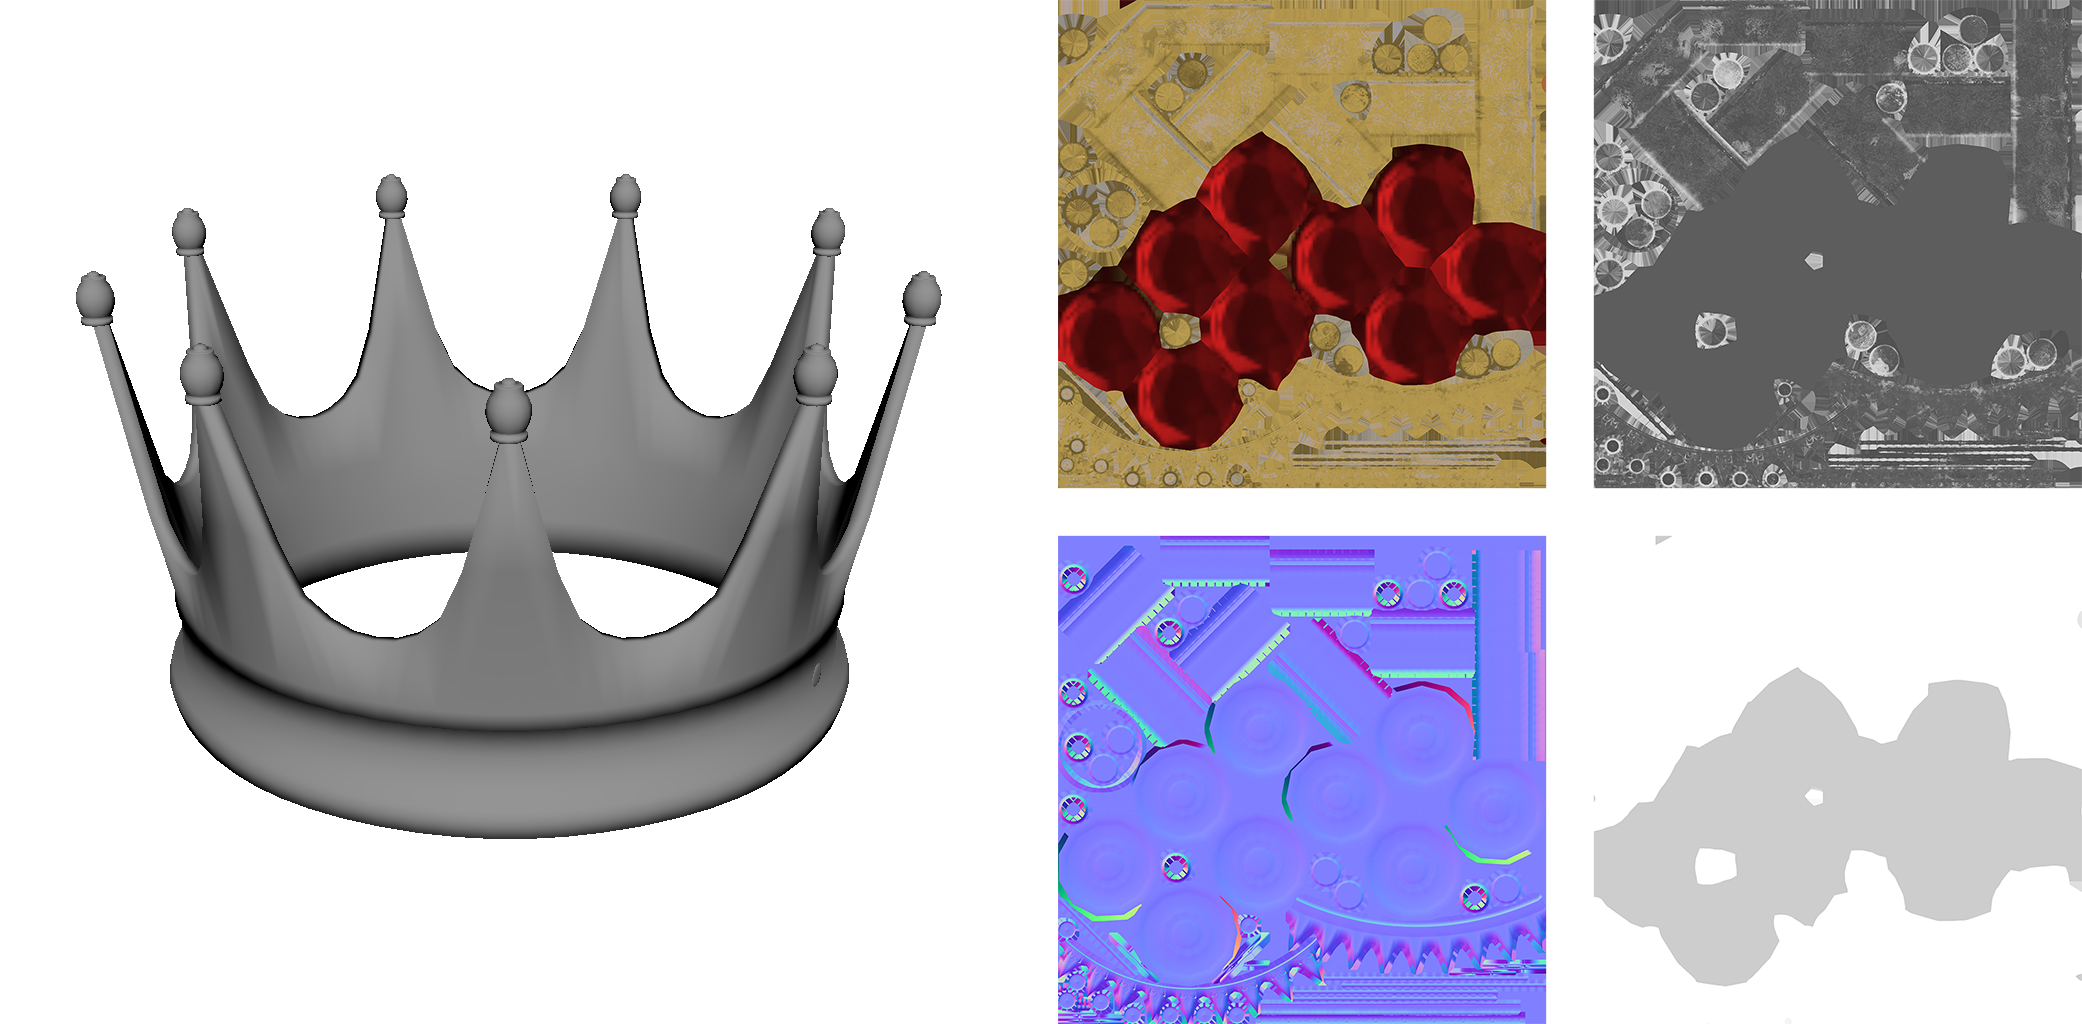
\includegraphics[height=3.5cm]{asset_error/digital_asset.png}
    \caption{数字资产皇冠}
  \end{subfigure}
  \hspace{3mm}
  \begin{subfigure}[t]{0.225\textwidth}
    \centering
    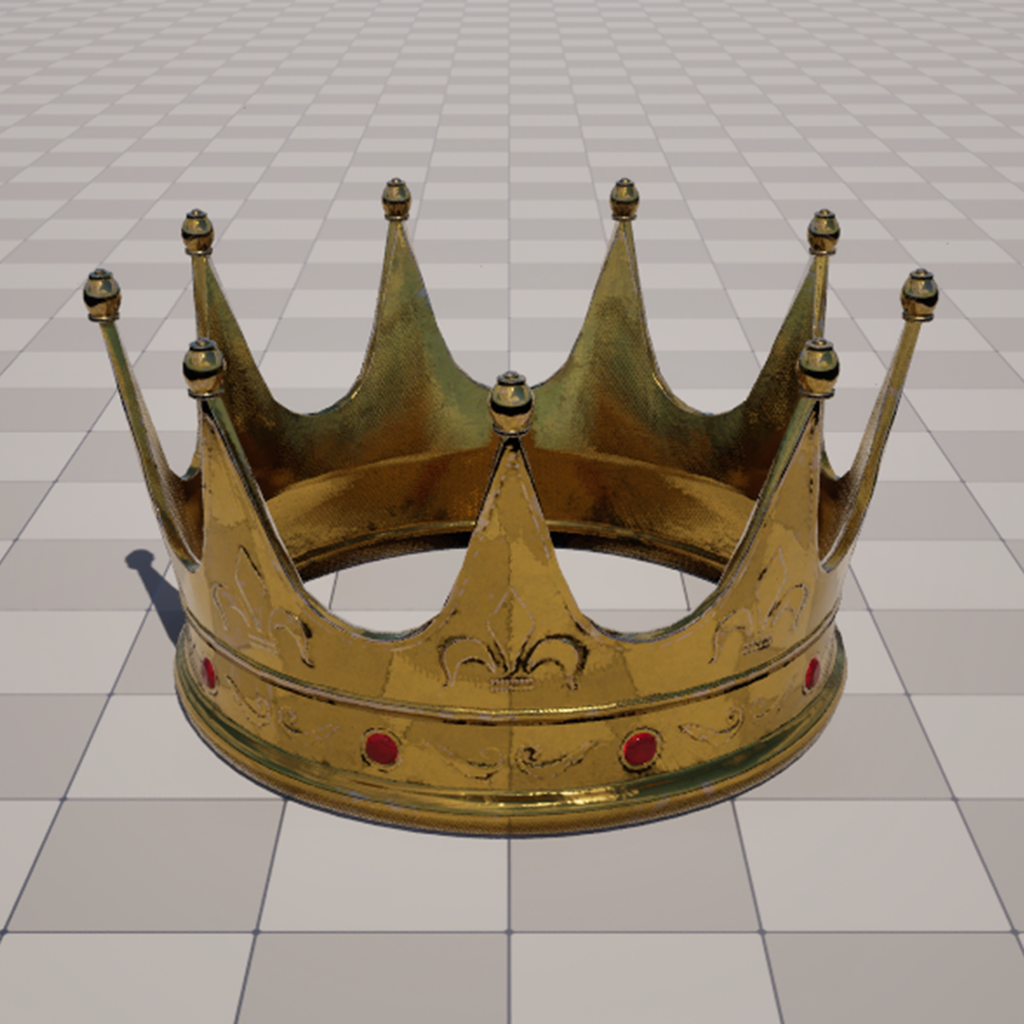
\includegraphics[height=3.5cm]{asset_error/correct.png}
    \caption{渲染结果}
  \end{subfigure}
  \begin{subfigure}[t]{0.225\textwidth}
    \centering
    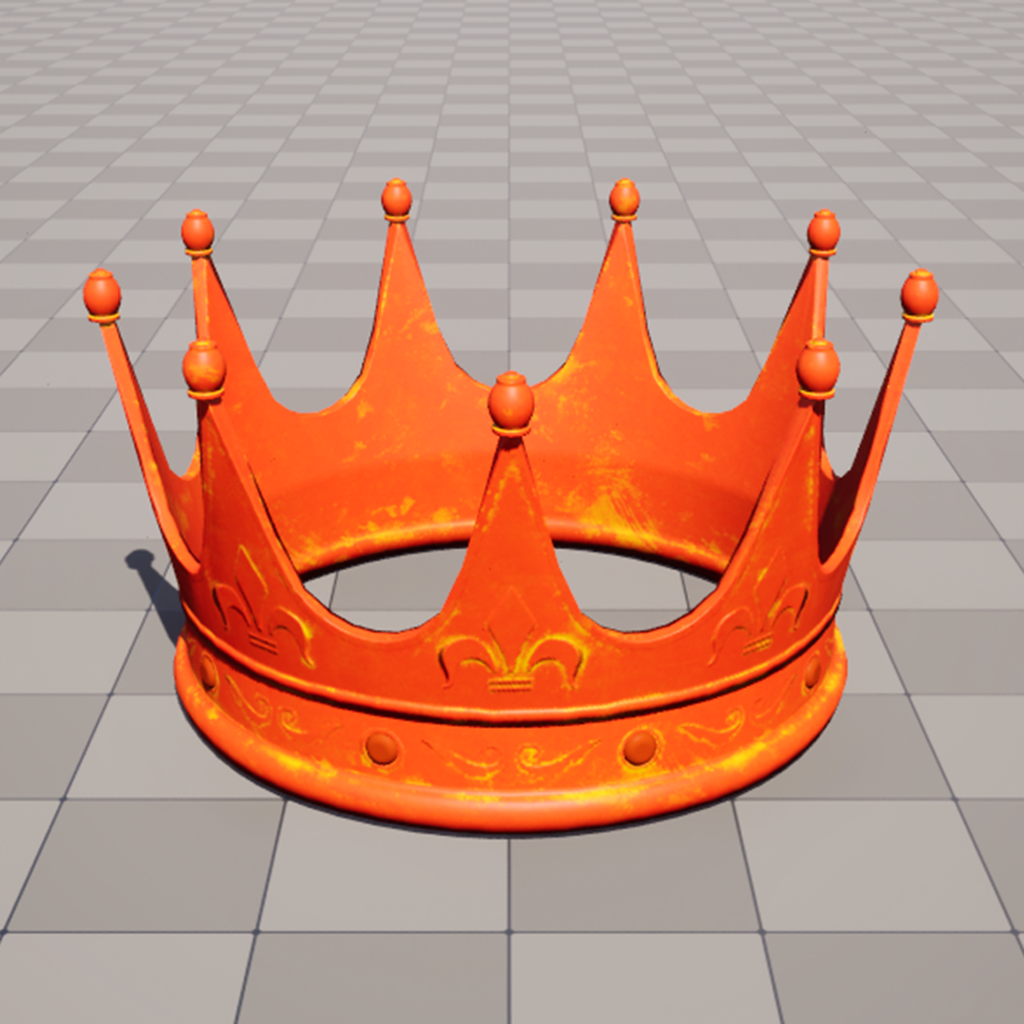
\includegraphics[height=3.5cm]{asset_error/error.png}
    \caption{渲染错误}
  \end{subfigure}
  \caption{数字资产及渲染}
  \label{fig:asset_rendering}
\end{figure}

为了尽可能减少二者耦合带来的负面影响,
在传统渲染管线中,不同领域和应用场景往往形成了各自的工作流(Workflow)。
工作流根据不同的渲染技术设计了不同的资产制作规范和后续编辑流程,在实际开发时,
资产只需严格遵循工作流的相应标准进行制作,即可保证能够兼容对应的渲染技术。

近年来,深度学习技术在计算机图形学领域崭露头角,
其中神经辐射场(Neural Radiance Fields,NeRF)作为一种新兴的三维场景表示方法,
通过隐式地将场景编码为连续的辐射场和体积密度场,实现了从稀疏二维图像重建三维场景的突破。
相较于传统方法,使用隐式连续表示的NeRF无需依赖显式的网格、点云或体素数据,避免了离散表示带来的伪影和内存开销,
展现了极高的通用性和灵活性。因此,本文旨在通过NeRF这种新颖的场景重建与表示技术,
解决数字资产与渲染技术之间紧密耦合的问题,为多种渲染工作流提供一种灵活、可编辑的数字资产表示方案。
本文的方法能够使得旧有资产不因技术不兼容被废弃,节省大量人力成本。
同时,也能允许开发者和创作者可以根据项目需求灵活切换工作流,提升创作自由度,
从而推动数字内容生产与渲染技术的发展。

\section{国内外研究现状}
\subsection{用于表征三维场景的神经辐射场}
NeRF通过多层感知机(Multilayer Perceptron,Coordinate-Based MLP)表示场景
并结合体积渲染生成新视角图像。传统方法
\cite{Waechter_2014, Mildenhall_2019, wu2020adversarial, Aliev_2020, Dai_2015}
通常采用显式的离散表示来构建三维场景,
但显式离散表示在利用梯度优化网格几何和拓扑结构时存在较大局限性,
因此研究者们逐渐转向基于连续体积的表示方案。
Mildenhall等人\cite{Mildenhall_2020}提出的NeRF采用了隐式的连续神经表示,用密度$\sigma$来描述场景几何形状,
通过光线步进在五维辐射场中计算出射辐射,从而实现图像渲染。
尽管这种方法在新视角合成上取得了令人印象深刻的成果,但由于体积渲染的固有局限,
NeRF生成的几何细节往往模糊不清,无法还原高频细节。

后续的相关研究主要集中在两个方向:一是探索改进的网络结构以保留更多场景细节
\cite{Chen_2022,Barron_2021,Barron_2022,dave2022pandora};
二是在不牺牲视觉质量的前提下,优化神经辐射场的训练与推理速度
\cite{Reiser_2021,Martin_Brualla_2021}。
同时,也有部分研究尝试采用基于表面的渲染方法,直接对物体表面进行优化。
例如,Wang等人\cite{10.5555/3540261.3542342}通过有向距离函数(Sign Distance Function,SDF)来表示形状,
并提出了从SDF到密度的无偏转换用以兼容NeRF的渲染框架。

然而,虽然以上这些方法在几何表示方法上各有不同,但仍然使用辐射场来描述场景的反射和光照信息。
辐射场将每一个着色点视为自发光光源,因此必须使用开销更高的体积渲染和光线步进生成图像,不兼容传统光栅化渲染器。
其次,这种编码方式使得NeRF相关研究易于完成新视角合成(Novel View Synthesis,NVS)任务,
但限制了NeRF在下游编辑任务或传统渲染器中的应用。


\subsection{神经辐射场的光照分解}

为了弥补上一节中所述的这些不足,Zhang等人\cite{Zhang_2021}和Boss等人\cite{Boss_2021}尝试将NeRF与可微渲染技术相结合,
在同一管线下联合优化,从而将辐射场信息分解为独立的几何形状、反射属性以及光照信息,以便在新的光照条件下实现重渲染或进一步编辑。
可微渲染旨在从观测图像中分离出物体的几何结构、材质属性和光照条件,将可微渲染融入NeRF框架的方案通常称为NeRF光照分解管线,
其研究重点在于如何准确地表示场景中的几何形状、反射属性和光照,以及如何选择合适的着色模型进行渲染。
下面将依次介绍现有方法在各个方面的研究现状。

\subsubsection*{(1)反射属性表示}

反射属性描述了光线在物体表面反射的特性。由于可微渲染为高度不适定(Highly ill-posed)的问题,
比如着色点颜色较亮既可能是由于粗糙浅色表面的漫反射产生,也可能是因为光滑深色表面的镜面反射导致,
因此早年间的工作\cite{Sato_1997, Zollh_fer_2015}中通常旨在恢复兰伯特(Lambertian)表面,即忽略掉高光反射属性。

近期工作\cite{Zhang_2023,10.5555/3600270.3601931}中多使用基于物理的着色模型,
其使用双向反射分布函数(Bidirectional reflectance distribution function,BRDF)
\cite{Cook_1981}来定义从反射属性到光照反射方式的计算过程。
NeRFactor\cite{zhang2021nerfactor}采用了数据驱动的BRDF,即将BRDF整体作为一个输出函数直接估计,
从而省略了将反射属性转换为BRDF的过程以降低误差。
Nerf2Mesh\cite{Tang_2023}则使用了近似的着色模型,抛弃了反射属性的物理意义,其管线的输出仅能使用特定的着色器。
这种方式虽然在一定程度上简化了问题,但导致输出的BRDF缺乏直观的物理意义,比如在传统渲染引擎中,
多采用参数化BRDF(如Disney Principled BRDF\cite{burley2012physically})使得材质编辑更加直观。
另外,由于基于物理的着色模型在真实感上的优越性能,所有的研究均采用了其或其近似。
但本文的目标旨在实现数字资产与渲染技术之间的解耦,数字资产可能需要多种着色模型进行渲染,
因此有必要对其进行扩展。为解决这些问题,本文提出的管线可以自定义不同的着色模型,
并通过材质管理的方式进行组织,以对应不同的工作流。这不仅使得输出结果能够直接用于传统渲染和后续编辑,
同时也实现了基于指定工作流的反射属性进行可微渲染的功能。

\subsubsection*{(2)几何形状表示}

几何形状表示的目标在于准确描述物体的空间结构和形态,为后续渲染与编辑奠定基础。
目前,大多数工作采用隐式神经表示来捕捉几何信息。虽然隐式神经表示在新视角合成任务中表现出色,
但其通常难以直接获得高质量的显式几何结构。其中,NeRD\cite{Boss_2021}维持了大部分原有的NeRF管线,
并且直接使用密度体积来表示几何形状。NeRFactor\cite{zhang2021nerfactor}在原有NeRF框架的基础上,
利用NeRF中的粗采样网络提取出神经表面,并在表面上进行后续的渲染步骤。
而其余大部分工作则根据NeuS\cite{10.5555/3540261.3542342}对NeRF的改进,使用SDF来表示几何形状,旨在还原更多高频细节,
如NeILF++\cite{Zhang_2023}、PhySG\cite{Zhang_2021}、NeRO\cite{Liu_2023}。然而这些工作使用的均为隐式神经表示,
主要面向重照明任务设计,而未专门针对下游编辑及传统渲染器渲染而优化。
针对这一局限,本文在NeRF光照分解任务中提出了一种基于混合几何表示方法的辐射场分解管线。
该方法能够将任意场景下的辐射场分解为显式表示的网格体,从而直接支持下游编辑任务与传统渲染技术。

\subsubsection*{(3)光照表示}

光照表示旨在描述场景中的光源分布、照明环境以及光与物体相互作用的方式,表示能力强的光照技术能够提升光照分解的效果,
而计算量较低的光照表示方法则可以降低优化的难度。
在可微渲染中,大多数工作都使用了近似的光照计算,以在优化难度和光照表示能力之间取得平衡。
NeRF-W\cite{martinbrualla2020nerfw}并未显式地表示光照,
而是使用嵌入向量表示不同场景的独有外观特征,以对齐不同光照环境中的场景,
这种方法虽然能够分离光照,但是无法使用其它光照技术进行重照明。
NeRF2Mesh\cite{Tang_2023}则重点针对几何体进行重建,因此没有使用独立建模的光照,
而是将光照表示和表面反射属性糅合在一起,牺牲掉重照明和材料编辑的能力以换取更好地几何体重建效果。
大多数现有方法使用近似的全局照明的方法计算光照,
例如PhySG\cite{Zhang_2021}和NeRD\cite{Boss_2021}使用的球面高斯(Spherical Gaussians,SGs),
其可以将复杂的全局光照转换为一组基函数的系数,大幅节省运算量。
与之类似的还有Lyu等人\cite{kuang2022neroic}利用球面谐波(Spherical Harmonics,SHs)计算光照。
Nvdiffrec-mc\cite{10.5555/3600270.3601931}直接优化环境贴图,并使用即时渲染中的近似技术进行加速。
这些全局照明技术均能满足可微渲染的要求,但大部分工作未能有效处理阴影与可见性问题。
NeRFactor虽然能够估计光源的可见性以建模阴影,
但其要求光照条件已知,并利用低分辨率环境图点光照\cite{zhang2021nerfactor}进行优化。
为了解决可微渲染中的光照无法高效表示阴影的问题,本文创新性地设计了一种基于条件输入的阴影调制模块,
能够将直接光照和环境光照根据阴影进行结合,并利用一个预训练的自动编码器定义了物理真实感和平滑的潜空间,
在不需要过高的额外计算成本的前提下提高了光照表示技术对阴影的处理能力。

\subsection{本文的主要贡献与创新}

本文设计的光照分解管线共为两个阶段,分别是利用NeRF建立神经辐射场,随后使用可微渲染分解神经辐射场,
最终获得指定标准的数字资产。本文的创新集中在1.2.2节所述的三个部分。针对光照表示,
本文设计了一种基于条件输入的阴影调制模块,并将其用于阴影感知的神经光照(Shadow-Aware Neural Light,SaNL),
创新地将直接光照和环境光照之间的关系融入其中,提升了光照方法的表示能力。在反射属性表示方面,
本文的管线允许根据工作流选择任意着色模型,赋予了管线输出任意工作流对应的数字资产的能力。
在几何形状表示方面,本文采用显式和隐式混合的表示方法,解决了现有研究仅能将结果用于重光照和新视角合成的问题,
实现了管线输出结果能够直接用于传统渲染和下游编辑。

总的来说,本文的贡献可以总结为:

\begin{itemize}
  \item 本文设计并实现了基于NeRF的数字资产解耦管线。该管线能够通过多张二维图像建立数字资产的神经表示,
  并以指定标准的工作流降维分解,解决了传统管线中数字资产与渲染技术之间的耦合,能够大幅节省游戏、影视等行业中的开发成本。
  \item 本文提出了阴影感知的神经光照表示SaNL,并使用即时渲染引擎和大量环境光照生成了阴影-光照数据集,训练了带有阴影关系、
  物理真实感和连续性等先验知识的神经光照表示。实验表明,在光照分解管线中,SaNL的表示效果优于现有的光照表示方式。
  \item 本文在管线中引入DMTet,实现了隐式和显式混合的几何形状表示方式,
  并设计了与其相匹配的损失函数以提高几何形状的分解效果。结合传统的纹理处理技术,
  本文的管线可以直接输出显式网格体表示的数字资产,无缝衔接了分解管线到传统的渲染任务或下游编辑。
\end{itemize}

\subsection{本文结构安排}
本节将介绍论文结构安排,包含每一章的主要内容和研究重点,以展示本文的工作思路和价值。

第1章,绪论。第1章首先介绍了本文工作的背景和意义,并进一步介绍了与本文研究相关的可微渲染研究、NeRF以及基于NeRF的光照分解。
本文根据以上研究的现状及本文目标,介绍了本文的创新点与主要贡献,并在最后一节阐述了全文的结构安排。

第2章,相关技术基础。在第2章中,本文将详细介绍工作内容相关的理论基础。为了理解NeRF和光照分解任务,
第2章首先将介绍深度学习的基本概念,然后深入讲解NeRF的理论基础。同时,第2章还介绍了传统管线中的概念及技术,
为本文管线与传统方法的对接打下了基础。最后,该章节将讨论可微渲染的理论基础,
为后续内容中进一步讲解本文研究提供理论支撑。

第3章,数字资产解耦管线的实现。第3章将介绍本文对数字资产解耦管线这一目标的具体实现。
本文首先通过分析选定了技术路线和工作内容。随后,本文解决了现有分解管线无法将输出直接用于传统渲染器的问题,
并引入了基于MLP的纹理来表示反射属性。最终本文实现了对数字资产解耦的目标,并完成了NeRF到传统渲染器和编辑的无缝衔接。
本文通过实验进一步证明了本文提出方法的适用性和可行性。

第4章,阴影感知的光照表示研究。第4章将介绍本文设计的用于表示光照的神经网络,
由于本文在第3章中观察到管线对阴影中的场景还原不加,因此创新性地设计了一种神经光照表示以解决该问题。
第4章从设计动机以及选用的基础结构出发,讲解本文创新性的阴影光照先验,并通过多个维度对该网络进行实验评估,以验证其有效性。

第5章,总结与展望。本章总结了全文的研究内容和成果,讨论了研究中的创新与不足,以及本文工作未来可能的改进方向和路线。

